% !TeX encoding = UTF-8

\chapter{MATERIAIS E MÉTODOS}\label{ch:materiais-metodos}
Após a revisão bibliográfica de outros estudos e os fundamentos teóricos necessários ....

Este capítulo apresenta os materiais e métodos utilizados ...


\section{TECNOLOGIAS E FERRAMENTAS}\label{sec: tec-ferramenta}
Tecnologias e ferramentas para a implementação de \textit{scripts} e utilização dos algoritmos.

%% Bibliotecas Python
\subsection{Bibliotecas da Linguagem Python}\label{sec:bib_python}
Um dos grandes diferenciais da linguagem Python é o seu enorme conjunto de bibliotecas para soluções de diversos problemas.

 
%%% sub: NumPy
\subsubsection{\textit{Biblioteca NumPy}}
\textit{NumPy} é o pacote fundamental para computação científica em Python. É o acrônico para \textit{Numerical Python}. Esta biblioteca provê:



%%% sub: pandas
\subsubsection{Biblioteca \textit{pandas}}\label{pandas}
A biblioteca \textit{pandas} ... \cite{python-analysis}:

Uma simples \textit{Series} é formado por uma única matriz de dados, conforme a \autoref{pandas-series}.

\begin{figure}[h!]
	\centering
	\fbox{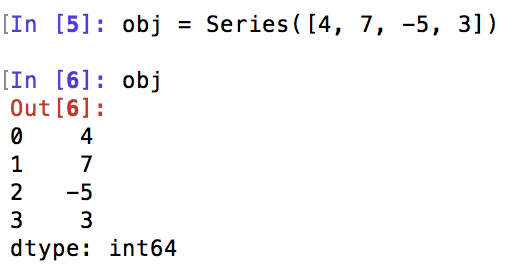
\includegraphics[width=.5\textwidth]{pandas-series}}
	\caption{Exemplo de uma \textit{Series}}
	\fonte{\citeonline{python-analysis}}
	\label{pandas-series}
\end{figure}

\textit{DataFrame} representa uma tabela...


% Twitter
\subsection{Rede Social \textit{Twitter}}
Para definir o que seria ...




\subsubsection{API do \textit{Twitter}}\label{api-twitter}
\textit{Twitter} é caracterizado como um serviço ...



% Bibliotecas Twitter
\subsubsection{Bibliotecas Para o Consumo de Dados da API do \textit{Twitter}}
O acesso a API acontece através da criação ....

O \autoref{cod:exempla-api} exemplifica o consumo da API segundo \citeonline{tweepy}.

\codigoPython
\lstinputlisting[label=cod:exempla-api, caption=Acesso à API do \textit{Twitter}]{src/acesso.py}





